

% Set up the document
\documentclass[convert={density=300,size=1080x800,outext=.png}]{standalone}

% Include any extra LaTeX packages required
%\usepackage[square, numbers, comma, sort&compress]{natbib}  % Use the "Natbib" style for the references in the Bibliography

\usepackage{verbatim}  % Needed for the "comment" environment to make LaTeX comments
\usepackage[table,x11names]{xcolor} % needed for highlighted rows

\usepackage{tabularx,booktabs,adjustbox} % For tables
\usepackage{pdflscape} % For writing some pages in landscape mode
\usepackage{afterpage} % For control over the positioning of figures and tables.

% For pictures
\usepackage{tikz}
\usetikzlibrary{calc,fit,arrows,decorations.pathmorphing,backgrounds,fit,positioning}
\usetikzlibrary{shapes.symbols}
 \usetikzlibrary{patterns}

% tikz colour settings
%\tikzset{pop0/.style={red!50!yellow},pop1/.style={violet!80},pop2/.style={olive!70!green}}

%% ----------------------------------------------------------------
\begin{document}

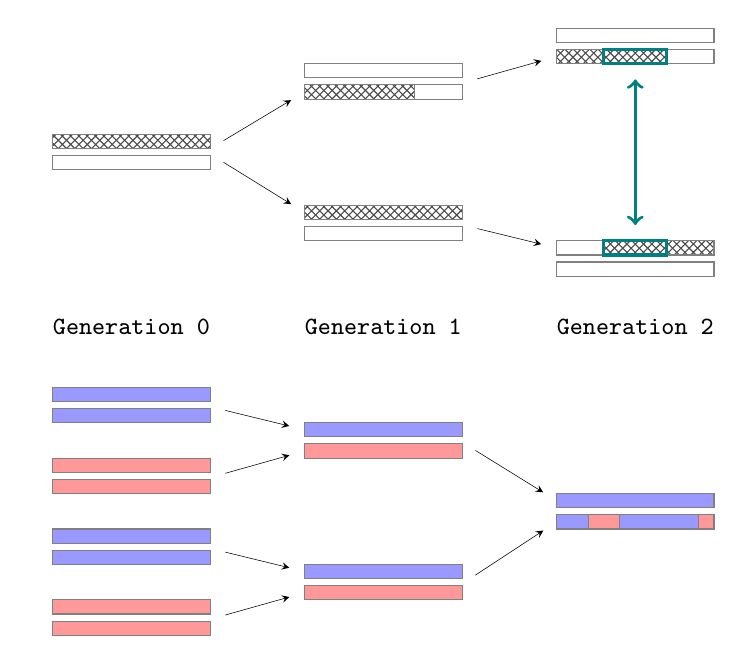
\begin{tikzpicture}[yscale=0.12, xscale=0.2]

\tikzset{
pop1/.style={fill=blue!40,draw=black!50},
pop2/.style={fill=red!40,draw=black!50},
ibd/.style={pattern=crosshatch,pattern color=black!70,draw=black!50},
nonibd/.style={fill=white,draw=black!50},
inherit/.style={->,>=stealth,ultra thin,shorten <=2mm,shorten >=2mm,very thin},
recomb/.style={thick,draw=black!70}
}

% Nodes
\node (hapx) at (1,0) {};
\node (hapy) at (0,1.5) {};
\node (hapxy) at ($10*(hapx) + (hapy)$) {};

\node (gen1) at (0,0) {};
\node (gen2) at ($8*(hapx) + 0*(hapx)$) {};
\node (gen3) at ($8*(hapx) + 8*(hapx)$) {};

\node (ind1gen3) at ($(gen3) + (0,0)$) {};
\node (indsep) at ($5*(hapy)$) {};

\node (ind1gen2) at ($(gen2) + 1*(indsep)$) {};
\node (ind2gen2) at ($(gen2) - 1*(indsep)$) {};

\node (ind1gen1) at ($(gen1) + 1.5*(indsep)$) {};
\node (ind2gen1) at ($(gen1) + 0.5*(indsep)$) {};
\node (ind3gen1) at ($(gen1) - 0.5*(indsep)$) {};
\node (ind4gen1) at ($(gen1) - 1.5*(indsep)$) {};

\node (chr1) at ($0.25*(hapy)$)  {};
\node (chr2) at ($-1.25*(hapy)$) {};


% Haplotypes

\filldraw[pop1] ($(gen1) + (ind1gen1) + (chr1)$) rectangle +(hapxy);
\filldraw[pop1] ($(gen1) + (ind1gen1) + (chr2)$) rectangle +(hapxy);

\filldraw[pop2] ($(gen1) + (ind2gen1) + (chr1)$) rectangle +(hapxy);
\filldraw[pop2] ($(gen1) + (ind2gen1) + (chr2)$) rectangle +(hapxy);

\filldraw[pop1] ($(gen1) + (ind3gen1) + (chr1)$) rectangle +(hapxy);
\filldraw[pop1] ($(gen1) + (ind3gen1) + (chr2)$) rectangle +(hapxy);

\filldraw[pop2] ($(gen1) + (ind4gen1) + (chr1)$) rectangle +(hapxy);
\filldraw[pop2] ($(gen1) + (ind4gen1) + (chr2)$) rectangle +(hapxy);


\filldraw[pop1] ($(gen2) + (ind1gen2) + (chr1)$) rectangle +(hapxy);
\filldraw[pop2] ($(gen2) + (ind1gen2) + (chr2)$) rectangle +(hapxy);

\filldraw[pop1] ($(gen2) + (ind2gen2) + (chr1)$) rectangle +(hapxy);
\filldraw[pop2] ($(gen2) + (ind2gen2) + (chr2)$) rectangle +(hapxy);


\filldraw[pop1] ($(gen3) + (ind1gen3) + (chr1)$) rectangle +(hapxy);
\fill[pop1] ($(gen3) + (ind1gen3) + (chr2)$) rectangle +(hapxy);
\fill[pop2] ($(gen3) + (ind1gen3) + (chr2)+ 2*(hapx)$) rectangle ($(gen3) + (ind1gen3) + (chr2)+ (hapxy)$);
\fill[pop1] ($(gen3) + (ind1gen3) + (chr2)+ 4*(hapx)$) rectangle ($(gen3) + (ind1gen3) + (chr2)+ (hapxy)$);
\fill[pop2] ($(gen3) + (ind1gen3) + (chr2)+ 9*(hapx)$) rectangle ($(gen3) + (ind1gen3) + (chr2)+ (hapxy)$);
%\draw ($(gen3) + (ind1gen3) + (chr2)$) rectangle +(hapxy);


% Copying lines

\node (startline) at ($-1*(hapx) + 0.5*(hapy)$) {};
\node (chrdiff) at ($(chr1) - (chr2)$) {};


% Arrows
\draw[inherit] ($(gen1) + (ind1gen1) + (chr2) + 10*(hapx) + 0.75*(chrdiff)$) -- ($(gen2) + (ind1gen2) + (chr1) + 0.5*(hapy)$);
\draw[inherit] ($(gen1) + (ind2gen1) + (chr2) + 10*(hapx) + 0.75*(chrdiff)$) -- ($(gen2) + (ind1gen2) + (chr2) + 0.5*(hapy)$);
\draw[inherit] ($(gen1) + (ind3gen1) + (chr2) + 10*(hapx) + 0.75*(chrdiff)$) -- ($(gen2) + (ind2gen2) + (chr1) + 0.5*(hapy)$);
\draw[inherit] ($(gen1) + (ind4gen1) + (chr2) + 10*(hapx) + 0.75*(chrdiff)$) -- ($(gen2) + (ind2gen2) + (chr2) + 0.5*(hapy)$);

\draw[inherit] ($(gen2) + (ind1gen2) + (chr2) + 10*(hapx) + 0.75*(chrdiff)$) -- ($(gen3) + (ind1gen3) + (chr1) + 0.5*(hapy)$);
\draw[inherit] ($(gen2) + (ind2gen2) + (chr2) + 10*(hapx) + 0.75*(chrdiff)$) -- ($(gen3) + (ind1gen3) + (chr2) + 0.5*(hapy)$);


% Labels
\node (lab1) at ($(gen1) + 2.5*(indsep) + 0.5*(hapxy)$) {\small $\texttt{Generation 0}$};
\node (lab2) at ($2*(gen2) + 2.5*(indsep) + 0.5*(hapxy)$) {\small $\texttt{Generation 1}$};
\node (lab3) at ($4*(gen2) + 2.5*(indsep) + 0.5*(hapxy)$) {\small $\texttt{Generation 2}$};

%%%%%%%%%%%%%%%%%%%%%
% Identity-by-descent
% Nodes
\node (hapx) at (1,0) {};
\node (hapyIBD) at (0,+38.0) {};
%\node (hapxy) at ($10*(hapx) + (hapy)$) {};

%\node (gen1) at (0,0) {};
%\node (gen2) at ($8*(hapx) + 0*(hapx)$) {};
%\node (gen3) at ($8*(hapx) + 8*(hapx)$) {};

%\node (indsep) at ($5*(hapy)$) {};
\node (ind1gen3) at ($(gen3) + 1.5*(indsep)$) {};
\node (ind2gen3) at ($(gen3) - 1.5*(indsep)$) {};

\node (ind1gen2) at ($(gen2) + 1*(indsep)$) {};
\node (ind2gen2) at ($(gen2) - 1*(indsep)$) {};

\node (ind1gen1) at ($(gen1) + 0*(indsep)$) {};

\node (chr1) at ($0.25*(hapy) + (hapyIBD)$)  {};
\node (chr2) at ($-1.25*(hapy)+ (hapyIBD)$) {};

% Haplotypes
\filldraw[ibd] ($(gen1) + (ind1gen1) + (chr1)$) rectangle +(hapxy);
\filldraw[nonibd] ($(gen1) + (ind1gen1) + (chr2)$) rectangle +(hapxy);

\filldraw[nonibd] ($(gen2) + (ind1gen2) + (chr1)$) rectangle +(hapxy);
\filldraw[ibd] ($(gen2) + (ind1gen2) + (chr2)$) rectangle +(hapxy);
\filldraw[nonibd] ($(gen2) + 7*(hapx) + (ind1gen2) + (chr2)$) rectangle ($(gen2) + (ind1gen2) + (chr2) + (hapxy)$);

\filldraw[ibd] ($(gen2) + (ind2gen2) + (chr1)$) rectangle +(hapxy);
%\filldraw[ibd] ($(gen2) + 3*(hapx) + (ind2gen2) + (chr1)$) rectangle ($(gen2) + (hapxy) + (ind2gen2) + (chr1)$);
\filldraw[nonibd] ($(gen2) + (ind2gen2) + (chr2)$) rectangle +(hapxy);

\filldraw[nonibd] ($(gen3) + (ind1gen3) + (chr1)$) rectangle +(hapxy);
\filldraw[ibd] ($(gen3) + (ind1gen3) + (chr2)$) rectangle +(hapxy);
\filldraw[nonibd] ($(gen3) + 7*(hapx) + (ind1gen3) + (chr2)$) rectangle ($(gen3) + (ind1gen3) + (chr2) + (hapxy)$);

\filldraw[nonibd] ($(gen3) + (ind2gen3) + (chr1)$) rectangle +(hapxy);
\filldraw[ibd] ($(gen3) + 3*(hapx) + (ind2gen3) + (chr1)$) rectangle ($(gen3) + (hapxy) + (ind2gen3) + (chr1)$);
\filldraw[nonibd] ($(gen3) + (ind2gen3) + (chr2)$) rectangle +(hapxy);

% Arrows
\draw[inherit] ($(gen1) + (ind1gen1) + (chr1) + 10*(hapx) + 0*(chrdiff)$) -- ($(gen2) + (ind1gen2) + (chr2) + 0.5*(hapy)$);
\draw[inherit] ($(gen1) + (ind1gen1) + (chr1) + 10*(hapx) - 0.25*(chrdiff)$) -- ($(gen2) + (ind2gen2) + (chr1) + 0.5*(hapy)$);

\draw[inherit] ($(gen2) + (ind1gen2) + (chr2) + 10*(hapx) + 0.75*(chrdiff)$) -- ($(gen3) + (ind1gen3) + (chr2) + 0.5*(hapy)$);
\draw[inherit] ($(gen2) + (ind2gen2) + (chr1) + 10*(hapx) - 0.25*(chrdiff)$) -- ($(gen3) + (ind2gen3) + (chr1) + 0.5*(hapy)$);

% IBD highlight.
\draw[color=teal,very thick] ($(gen3) + (ind1gen3) + (chr2) + 3*(hapx)$) rectangle +($4*(hapx) + (hapy)$);
\draw[color=teal,very thick] ($(gen3) + (ind2gen3) + (chr1) + 3*(hapx)$) rectangle +($4*(hapx) + (hapy)$);
\draw[color=teal,very thick,<->,shorten <=2mm,shorten >=2mm] ($(gen3) + (ind1gen3) + (chr2) + 5*(hapx)$) -- ($(gen3) + (ind2gen3) + (chr1) + 5*(hapx) + (hapy)$) ; 

\end{tikzpicture}
\end{document}  % The End
%% ----------------------------------------------------------------